\section{AWS EC2 Container Service}
Deploying an app to EC2 Container service consisted of deploying the following service an infrastructure:
\begin{itemize}
	\item ECS Cluster
	\item ECS Optimized EC2 Instance
	\item Task Definition
	\item Application Load Balancer \& Target Group
	\item Service
	\item Application Autoscaling
	\item Scaling Policies \& Cloudwatch Alarms
\end{itemize}
The topology is shown below in \autoref{fig:topology}

\begin{figure}[H]
	\setlength{\belowcaptionskip}{15pt plus 3pt minus 2pt}
	\caption{Topology}
	\centering
	%\includegraphics[width=\textwidth,height=\textheight,keepaspectratio]{diagram}
	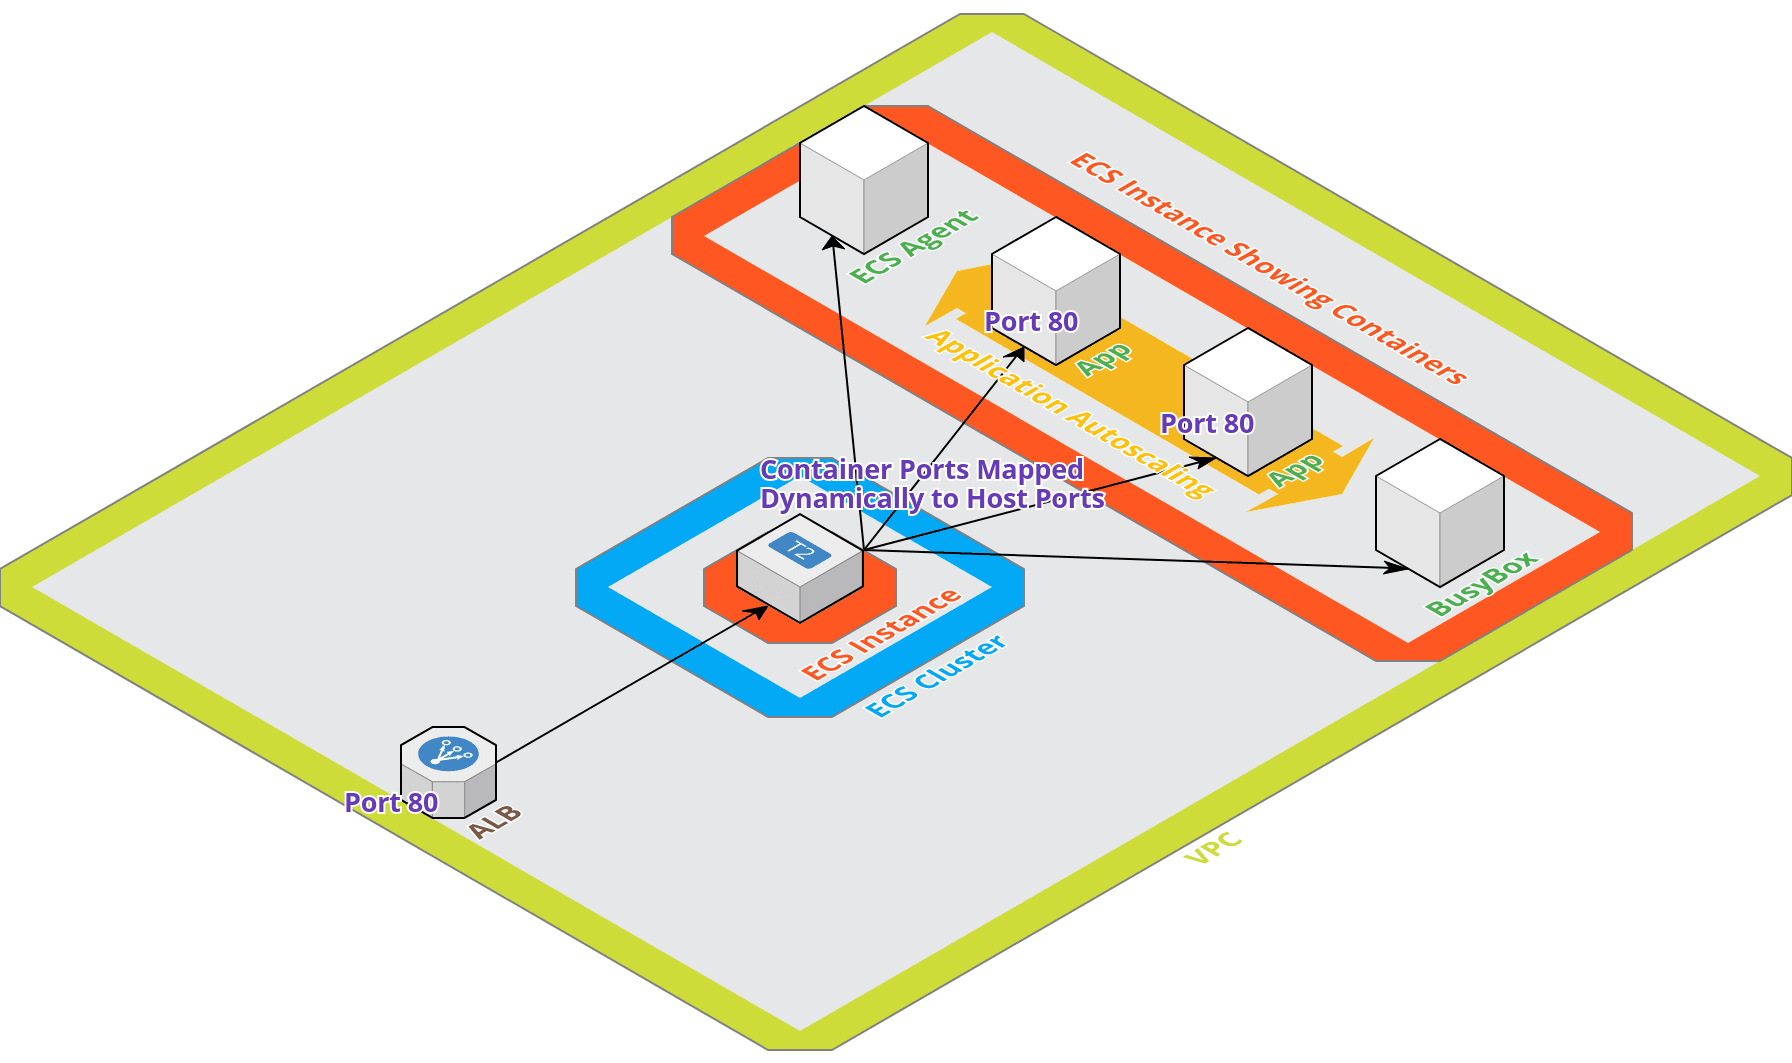
\includegraphics[width=\textwidth,keepaspectratio]{ecs-topology}
	\label{fig:topology}
\end{figure}

\subsection{Setting up the ECS}
The first step was to create an ECS cluster and an instance:
\begin{lstlisting}[language=bash]
aws ecs create-cluster --cluster-name $CLUSTER_NAME
aws ec2 run-instances --image-id $AMI_ID --count 1 --instance-type t2.micro --key-name $KEY_NAME --security-groups $HTTPSSH_SEC_GROUP $VPC_SEC_GROUP --iam-instance-profile Name=$ECS_INSTANCE_ROLE --user-data file://files/user-data.txt --tag-specifications 'ResourceType=instance,Tags=[{Key=Name,Value='$INSTANCE_NAME'}]'
\end{lstlisting}
There are some important parameters to notice here. \textbf{Image ID} is used to specify that an image optimised for ECS is used for the instance. This means that an ECS container agent will be installed and run on the image. The agent allows the instance to connect to a cluster.

The \textbf{VPC Security Group} is used to allow traffic to the instance from it's own VPC. This will be of importance when the application load balancer is added.

\textbf{User Data} is used to specify which cluster to add the instance to. The cluster is a group of ECS instances. Although only one instance will be used in this topology, the cluster allows for application load balancer to occur over many containers over many instances. User data is shown is appendix \ref{user-data}).


Next a task definition is created.
\begin{lstlisting}[language=bash]
aws ecs register-task-definition --cli-input-json file://simple-app-task-def.json
\end{lstlisting}

A task definition contains instructions for running a container on the instance.  It specifies the image to run and where to pull the image from (i.e ECS registry or an external registry such Docker Hub. The task definitions used specifies the simple php-app contained on Docker Hub. It also details port numbers to be used. For this implementation, in which an application load balancer and multiple container apps will be used, the task definition specifies that the container should use port 80. It also specifies that the host port used should be 0. This will dynamically map a random port number of the host to port 80 the container. This is necessary because multiple container apps will run on the instance so they cannot all be accessed via port 80. The task definition can be seen in appendix \ref{task-definition}.
Also detailed in the task definition is the resources allocated to each container. In order to allow all the necessary containers to run on the \textit{t2.micro} used in this topology, tall containers were allocated 100MiB, including the \textit{BusyBox} container.

\subsection{Load Balancing}
Load balancing is achieved using an Application load balancer (ALB). The an ALB has the ability to balance traffic across multiple apps running in multiple containers on one or more instances.
\begin{lstlisting}[language=bash]
aws elbv2 create-load-balancer --type application --name $LB_NAME --security-groups $HTTPSSH_SEC_GROUP_ID $VPC_SEC_GROUP_ID --subnets $SUBNET_A_ID $SUBNET_B_ID $SUBNET_C_ID
\end{lstlisting}
A target group is also created and the instance registered one it. This tell the ALB where to route traffic.
\begin{lstlisting}[language=bash]
aws elbv2 create-target-group --name $TG_NAME --protocol HTTP --port 80 --vpc-id $VPC_ID --target-type instance --health-check-protocol HTTP --health-check-path "/index.php"
aws elbv2 register-targets --target-group-arn $TG_ARN --targets Id=$INSTANCE_ID
\end{lstlisting}
The target group is the instance on which the containers are running. It registers the app containers as targets for the ALB via the host port numbers which have been dynamically allocated according to the task definition (as mentioned above). It also monitors the health of the containers health check.

An listener is added to the ALB and configured to use the target group. This listens on the configured port (80 in this case) of the ALB and routes traffic to the correct ports for the app containers (registered through the instance to the target group).
\begin{lstlisting}[language=bash]
aws elbv2 create-listener --load-balancer-arn $LB_ARN --protocol HTTP --port 80 --default-actions Type=forward,TargetGroupArn=$TG_ARN
\end{lstlisting}
The ALB has been configured with a security that allows inbound HTTP traffic. This allows web browser to view the app using the ALBs address. However, as described, the ALB routes traffic to the app containers on the dynamically allocated port numbers. It can't direct traffic to numerous containers all using port 80. Therefore, the same security group won't allow traffic to the instance, and therefore will prevent the apps displaying when visiting the ALBs address. This is the reason the VPC security group was used when creating the instance above. The instance will allow traffic from inside it's own VPC, which includes the ALB.

\subsection{Service}
The service is used to scale the web app. If only a single container running the web app was needed a service would not be required (or the ALB) and the task definition created above could be run (using host port 80). However a service can be used to run multiple task definitions behind the ALB according to an application autoscaling policy. The ECS instance is registered and a scalable target for service.
\begin{lstlisting}[language=bash]
aws ecs create-service --cluster $CLUSTER_NAME --service-name $SERVICE_NAME --task-definition $TASK_DEF:$REVISION --load-balancers targetGroupArn=$TG_ARN,containerName=$CONTAINER_NAME,containerPort=80 --desired-count 2 --role $ECS_SERVICE_ROLE
aws application-autoscaling register-scalable-target --service-namespace ecs --resource-id service/$CLUSTER_NAME/$SERVICE_NAME --scalable-dimension ecs:service:DesiredCount --min-capacity 1 --max-capacity 3 --role-arn $APP_AUTOSCALING_ROLE_ARN
\end{lstlisting}
Once the service is created with a desired number of task set to a number greater than zero and application autoscaling is configure, the service will automatically start the desired number of instance. I.e. Autoscaling will not occur because there are no policies configured than simple scaling to the desired number of tasks. The app can now be view through the ALB ash shown in \autoref{fig:app}

\begin{figure}[H]
	\setlength{\belowcaptionskip}{15pt plus 3pt minus 2pt}
	\caption{Simple Web App Running Behind Application Load Balancer}
	\centering
	%\includegraphics[width=\textwidth,height=\textheight,keepaspectratio]{diagram}
	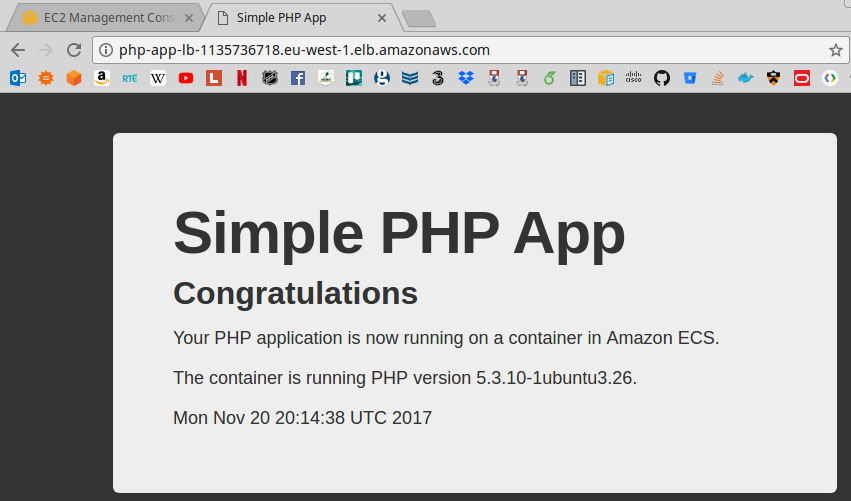
\includegraphics[width=\textwidth,keepaspectratio]{php-app-working}
	\label{fig:app}
\end{figure}


\subsection{Application Autoscaling}
Finally the scaling policies and their corresponding cloudwatch alarms are created for the application autoscaling.
This consists of three main components, the scaling policies, scaling actions and cloud watch alarms.
First the scaling policies are defined. This defines the scalable resource, i.e. the desired count of the service and the type of scaling to implement (Step scaling in this case).
\begin{lstlisting}[language=bash]
aws application-autoscaling put-scaling-policy --policy-name $SCALE_OUT_POLICY_NAME  --service-namespace ecs --resource-id service/$CLUSTER_NAME/$SERVICE_NAME --scalable-dimension ecs:service:DesiredCount --policy-type StepScaling --step-scaling-policy-configuration="AdjustmentType=ChangeInCapacity,StepAdjustments=[{ScalingAdjustment=0,MetricIntervalLowerBound=0}],MetricAggregationType=Average,Cooldown=60"
aws application-autoscaling put-scaling-policy --policy-name $SCALE_IN_POLICY_NAME  --service-namespace ecs --resource-id service/$CLUSTER_NAME/$SERVICE_NAME --scalable-dimension ecs:service:DesiredCount --policy-type StepScaling --step-scaling-policy-configuration="AdjustmentType=ChangeInCapacity,StepAdjustments=[{ScalingAdjustment=0,MetricIntervalLowerBound=0}],MetricAggregationType=Average,Cooldown=60"
\end{lstlisting}
Then the cloudwatch alarms are created. These monitor some resource, CPU utilisation in this case, and trigger actions when certain limits are met. 
\begin{lstlisting}[language=bash]
aws cloudwatch put-metric-alarm --alarm-name $SCALE_OUT_ALARM_NAME --metric-name CPUUtilization --namespace AWS/ECS --statistic Average --dimensions "Name=ClusterName,Value=php-app Name=ServiceName,Value=php-app-service" --period 60 --evaluation-periods 60 --comparison-operator GreaterThanOrEqualToThreshold --threshold 75 --unit Percent --actions-enabled --alarm-actions $SCALE_OUT_POLICY_ARN
aws cloudwatch put-metric-alarm --alarm-name $SCALE_IN_ALARM_NAME --metric-name CPUUtilization --namespace AWS/ECS --statistic Average --dimensions "Name=ClusterName,Value=php-app Name=ServiceName,Value=php-app-service" --period 60 --evaluation-periods 60 --comparison-operator LessThanOrEqualToThreshold --threshold 25 --unit Percent --actions-enabled --alarm-actions $SCALE_IN_POLICY_ARN
\end{lstlisting}
However, while completing this exercise it was noted that configuring a scalable action for a namespace of AWS ECS was impossible using the CLI. Therefore this step was carried out though the AWS console.
